\documentclass[a4paper,12pt]{article} 

%%% Работа с русским языком
\usepackage{cmap}					% поиск в PDF
\usepackage{mathtext} 				% русские буквы в фомулах
\usepackage[T2A]{fontenc}			% кодировка
\usepackage[utf8]{inputenc}			% кодировка исходного текста
\usepackage[english,russian]{babel}	% локализация и переносы

%%% Дополнительная работа с математикой
\usepackage{amsmath,amsfonts,amssymb,amsthm,mathtools, gensymb} % AMS
\usepackage{icomma} % "Умная" запятая: $0,2$    ф--- число, $0, 2$ --- перечисление

%%Таблица
\usepackage[table,xcdraw]{xcolor}
\usepackage{caption}
\usepackage{floatrow}
\floatsetup[table]{capposition=top}
\floatsetup[wrapfigure]{capposition=bottom}
\usepackage{multirow}

%Отступы и поля 
\textwidth=18cm
\oddsidemargin=-1cm
\topmargin=-2cm
\textheight=25cm


%% Номера формул
\mathtoolsset{showonlyrefs=true} % Показывать номера только у тех формул, на которые есть \eqref{} в тексте.

%% Шрифты
\usepackage{euscript}	 % Шрифт Евклид
\usepackage{mathrsfs} % Красивый матшрифт

%% Свои команды
\DeclareMathOperator{\sgn}{\mathop{sgn}}

%% Перенос знаков в формулах (по Львовскому)
\newcommand*{\hm}[1]{#1\nobreak\discretionary{}
{\hbox{$\mathsurround=0pt #1$}}{}}

%% Стиль страницы
\usepackage{fancyhdr}

%% Для рисунков
\usepackage{graphicx}
\usepackage[export]{adjustbox}
\usepackage{float}
\usepackage{ragged2e}
\usepackage{wrapfig}

\pagestyle{fancy}
\begin{document}
\begin{titlepage}
\begin{center}
%\vspace*{1cm}
\large{\small ФЕДЕРАЛЬНОЕ ГОСУДАРСТВЕННОЕ АВТОНОМНОЕ ОБРАЗОВАТЕЛЬНОЕ\\ УЧРЕЖДЕНИЕ ВЫСШЕГО ОБРАЗОВАНИЯ \\ МОСКОВСКИЙ ФИЗИКО-ТЕХНИЧЕСКИЙ ИНСТИТУТ\\ (НАЦИОНАЛЬНЫЙ ИССЛЕДОВАТЕЛЬСКИЙ УНИВЕРСИТЕТ)\\ ФАКУЛЬТЕТ АЭРОКОСМИЧЕСКИХ ТЕХНОЛОГИЙ}
\vfill
\line(1,0){490}\\[1mm]
\huge{Лабораторная работа 4.3.1}\\
\huge\textbf{Изучение дифракции света}\\
\line(1,0){490}\\[1mm]
\vfill
\begin{flushright}
\normalsize{Рогозин Владимир}\\
\normalsize{\textbf{Группа Б03-106}}\\
\end{flushright}
\end{center}
\end{titlepage}
\fancyhead[L] {Работа 4.3.1}

\textbf{Цель работы}:
исследовать явления дифракции Френеля и Фраунгофера на щели, изучить влияние дифракции на разрешающую способность оптических инструментов.


\textbf{Оборудование}:
В работе используются: оптическая скамья, ртутная лампа, монохроматор, щели с регулируемой шириной, рамка с вертикальной нитью, двойная щель, микроскоп на поперечных салазках с микрометрическим винтом, зрительная труба.

\section{Теоретические сведения}
\subsection{Дифракция Френеля на щели}

\begin{figure}[H]\label{fig: Fresnel diffraction setup}
    \centering
    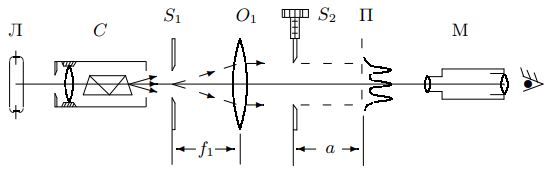
\includegraphics[width = 0.9\textwidth]{Fresnel diffraction setup.png}
    \caption{ Схема установки для наблюдения дифракции Френел}
\end{figure}
Схема установки для наблюдения дифракции Френеля представлена на рис. 1. Световые лучи освещают щель $S_2$ и испытывают на ней дифракцию. Щель $S_2$ освещается параллельным пучком монохроматического света с помощью коллиматора, образованного объективом $O_1$ и щелью $S_1$, находящейся в его фокусе. На щель $S_1$ сфокусировано изображение спектральной линии, выделенной из спектра ртутной лампы $Л$ при помощи простого монохроматора $C$, в котором используется призма прямого зрения. 

\begin{wrapfigure}[17]{l}{0.4\textwidth}\label{fig: Schuster zones}
    \begin{center}
    \vspace{-20pt}
        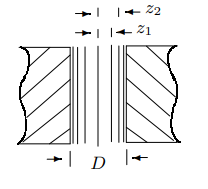
\includegraphics[width = 0.9\textwidth]{Schuster zones.png}
    \end{center}
    \caption{Зоны Френеля в плоскости щели}
\end{wrapfigure}
Распределение интенсивности света в плоскости наблюдения $П$ проще всего рассчитывать с помощью зон Шустера. При освещении щели $S_2$ параллельным пучком лучей (плоская волна) зоны Френеля представляют собой полоски, параллельные краям щели (рис. 2). Результирующая амплитуда в точке наблюдения определяется суперпозицией колебаний от тех зон Френеля, которые не перекрыты створками щели. Графическое определение результирующей амплитуды производится с помощью спирали Корню. Суммарная ширина $m$ зон Френеля $z_m$ определяется соотношением
\begin{equation}\label{eq: first m Schuster zones' width}
    z_m = \sqrt{am\lambda},
\end{equation}
где $a$ -- расстояние от щели до плоскости наблюдения, а $\lambda$ -- длина волны.

Вид наблюдаемой дифракционной картины определяется \textit{числом Френеля} $\Phi$: квадрат которого 
\begin{equation}\label{eq: Fresnel number}
    \Phi^2 = \frac{D}{\sqrt{a\lambda}}
\end{equation}
-- это отношение ширины щели $D$ к размеру первой зоны Френеля, т.е. число зон Френеля, которые укладываются на ширине щели. Обратную величину называют \textit{волновым параметром}
\begin{equation}\label{eq: Wave parameter}
    p = \frac{1}{D^2} = \frac{\sqrt{a\lambda}}{D}.
\end{equation} 
Дифракционная картина отсутствует, когда плоскость наблюдения $П$ совпадает с плоскостью щели: при $\Phi \rightarrow \infty$ мы имеем дело с геометрической оптикой. При небольшом
удалении от щели, когда число Френеля $\Phi \gg 1$, распределение интенсивности света за щелью также можно получить с помощью законов геометрической оптики (приближённо). Дифракционная картина в этом случае наблюдается только в узкой области на границе света и тени у краёв экрана.

При последующем небольшом удалении от щели (или изменении ширины щели $S_2$) эти две группы дифракционных полос перемещаются практически независимо друг от друга. Каждая из этих групп образует картину дифракции Френеля на краю экрана. Распределение интенсивности при дифракции света на краю экрана может быть найдено с помощью спирали Корню.

При дальнейшем увеличении расстояния $a$ (или уменьшении ширины щели $S_2$) обе системы дифракционных полос постепенно сближаются и, наконец, при $\Phi \approx 1$ накладываются друг на друга. Распределение интенсивности в плоскости наблюдения в этом случае определяется числом зон Френеля, укладывающихся на полуширине щели. Если это число равно $m$, то в поле зрения наблюдается $n = m - 1$ тёмных полос. Таким образом, по виду дифракционной картины можно оценить число зон Френеля на полуширине щели.

\subsection{Дифракция Фраунгофера на щели}

\begin{wrapfigure}[17]{l}{0.4\textwidth}\label{fig: Frauhofer phase difference}
    \begin{center}
    \vspace{-20pt}
        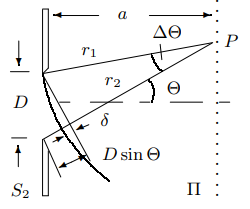
\includegraphics[width = 0.9\textwidth]{Fraunhofer diffraction phase difference.png}
    \end{center}
    \caption{К фазовым соотношениям при дифракции Фраунгофера}
\end{wrapfigure}
Картина дифракции резко упрощается, когда ширина щели становится значительно меньше ширины первой зоны Френеля, т.е. если 
\begin{equation}\label{eq: Fraunhofer condition}
    D \ll \sqrt{a\lambda} \quad \text{или} \quad \Phi \ll 1.
\end{equation}
Это условие всегда выполняется при достаточно большом расстоянии $a$ от щели до плоскости наблюдения. Дифракционную картину, наблюдаемую в этом случае, принято называть \textit{дифракцией Фраунгофера}. Исследование такой дифракционной картины заметно облегчается, потому что упрощаются фазовые соотношения. При выполнении условия \eqref{eq: Fraunhofer condition} разность хода между крайними лучами, приходящими от щели в точку наблюдения $P$, с хорошим приближением можно вычислять по формуле
\begin{equation}\label{eq: Delta Frauhofer diffraction}
    \Delta = r_2 - r_1 \approx D \sin\Theta \approx D \cdot \Theta.
\end{equation}

Здесь предполагается, что дифракционный угол $\Theta$ достаточно мал, так что $\sin\Theta \approx \Theta$. Формула \eqref{eq: Delta Frauhofer diffraction} справедлива при условии $\delta \ll \lambda / 2$. Это условие эквивалентно условию \eqref{eq: Fraunhofer condition}.

Дифракцию Френеля и Фраунгофера можно наблюдать на одной и той же установке (рис. 1). Однако при обычных размерах установки дифракция Фраунгофера возникает только при очень узких щелях. Поскольку работать с такими тонкими щелями неудобно, для наблюдения
дифракции Фраунгофера к схеме, изображённой на рис. 1 добавляется объектив $O_2$ (рис. 4)

\begin{figure}[H]\label{fig: Fraunhofer diffraction setup}
    \centering
    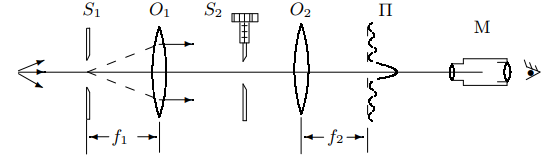
\includegraphics[width = 0.9\textwidth]{Fraunhofer diffraction setup.png}
    \caption{   Схема установки для наблюдения дифракции Фраунгофера на щели}
\end{figure}

\begin{wrapfigure}[17]{r}{0.5\textwidth}\label{fig: Fraunhofer diffraction intensity}
    \begin{center}
    \vspace{-20pt}
        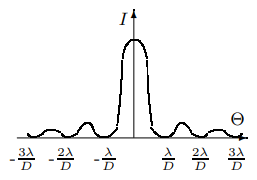
\includegraphics[width = 0.9\textwidth]{Fraunhofer diffraction intensity.png}
    \end{center}
    \caption{Распределение интенсивности при дифракции Фраунгофера на щели}
\end{wrapfigure}
Дифракционная картина наблюдается здесь в фокальной плоскости объектива $O_2$. Каждому значению угла $\Theta$ соответствует в этой плоскости точка, отстоящая от оптической
оси на расстоянии
\begin{equation}\label{eq: Fraunhofer diffraction X via Theta}
    X = f_2 \cdot\text{ tg}\Theta \approx f_2 \Theta.
\end{equation}

Поскольку объектив не вносит дополнительной разности хода между интерферирующими лучами (таутохронизм), в его фокальной плоскости наблюдается неискажённая дифракционная картина Фраунгофера. Эта картина соответствует бесконечно удалённой плоскости наблюдения. Распределение интенсивности в дифракционной картине Фраунгофера представлено на рис. 5.

Поскольку при $\Theta = 0$ разность хода между любой парой лучей равна нулю, в центре поля зрения наблюдается дифракционный максимум. Первый минимум соответствует такому значению дифракционного угла $\Theta_1$, при котором в точке наблюдения разность хода пробегает все возможные значения от нуля до $2\pi$. Таким образом, можно определить угловую координату $\Theta_m$ любой тёмной полосы. Для малых углов
\begin{equation}\label{eq: Fraunhofer diffraction min intensity Theta}
    m\lambda = D \cdot \Theta_m.
\end{equation}
Расстояние $X_m$ тёмной полосы от оптической оси объектива $O_2$ пропорционально фокусному расстоянию $f_2$. Из \eqref{eq: Fraunhofer diffraction X via Theta} и \eqref{eq: Fraunhofer diffraction min intensity Theta} следует
\begin{equation}\label{eq: Fraunhofer diffraction min intensity X}
    X_m = f_2m\frac{\lambda}{D}.
\end{equation}
Из \eqref{eq: Fraunhofer diffraction min intensity X} видно, что при малых углах минимумы эквидистантны, а расстояния $\Delta X$ между минимумами обратно пропорциональны ширине $D$ щели $S_2$.

\subsection{Дифракция Фраунгофера на двух щелях}

Для наблюдения дифракции Фраунгофера на двух щелях в установке (рис. 4) следует заменить щель
$S_2$ экраном $Э$ с двумя щелями (рис. 6). При этом для оценки влияния ширины входной щели на чёткость дифракционной картины вместо входной щели $S_1$ следует поставить щель с микрометрическим винтом. Два дифракционных изображения входной щели, одно из которых образовано лучами, прошедшими через левую, а другое -- через правую щели, накладываются друг на друга.

Если входная щель достаточно узка, то дифракционная картина в плоскости $П$ (рис. 6) подобна той, что получалась при дифракции на одной щели (рис. 4), однако теперь вся картина испещрена рядом дополнительных узких полос. Наличие этих полос объясняется суперпозицией световых волн, приходящих в плоскость наблюдения через разные щели экрана $Э$. В центре главного дифракционного максимума (рис. 6) располагается светлая полоса, так как при $\Theta = 0$ разность хода между этими волнами равна нулю. Светлая интерференционная полоса наблюдается и во всех тех случаях, когда указанная разность хода равна целому числу длин волн. Таким образом, угловая координата $\Theta_m$ интерференционного максимума $m$-го порядка определяется соотношением
\begin{equation}\label{eq: Fraunhofer diffraction 2 Theta max}
    d \cdot \Theta_m = m\lambda,
\end{equation}
где $d$ -- расстояние между щелями.

Линейное расстояние $\delta x$ между соседними интерференционным и полосами в плоскости $П$ равно поэтому
\begin{equation}\label{eq: Fraunhofer diffraction 2 deltaX}
    \delta x = f_2 \frac{\lambda}{d}.
\end{equation}

На рис. 6 показано распределение интенсивности в фокальной плоскости объектива
$O_2$.

Нетрудно оценить число $n$ интерференционных полос, укладывающихся в области центрального дифракционного максимума. Согласно \eqref{eq: Fraunhofer diffraction min intensity X} полная ширина главного максимума равна $2f_2\lambda /D$, где D -- ширина щели, отсюда
\begin{equation}\label{eq: Fraunhofer diffraction 2 n in first max}
    n = \frac{2\lambda f_2}{D}\frac{1}{\delta x} = \frac{2d}{D}.
\end{equation}

При дифракции света на двух щелях чёткая система интерференционных полос наблюдается только при достаточно узкой ширине входной щели $S$. При увеличении её ширины интерференционная картина периодически пропадает и появляетс я вновь, но полосы при этом оказываются сильно размытыми и видны плохо. Это явление объясняется наложением интерференционных картин от разных элементов широкой щели
$S$. Первое размытие интерференционных полос возникает при условии
\begin{equation}\label{eq: Fraunhofer 2 diffraction first blur}
    \frac{b}{f_1} = \frac{\lambda}{d}.
\end{equation}
Здесь $b$ -- ширина входной щели $S$ и, следовательно, $b/f_1$ — её угловая ширина. Таким образом, по размытию интерференционной картины можно оценить размер источника. Этот метод используется в звёздном интерферометре при измерении угловых размеров звёзд.
 
%\section{Экспериментальная установка}

\section{Обработка данных} 
В данной работе все измерения были проведены на монохроматическом свете длины волны $\lambda = 546,1$ нм.
\subsection{Дифракция Френеля на щели}
\begin{enumerate}
    \item
    Соберём схему согласно рис. 1.

    \item
    Установим линзу $O_1$ на расстоянии от щели $S_1$, близком к фокусному $f = 12,5$ см. 

    \item
    Далее настроим зрительную трубу на бесконечность с помощью удалённого объекта (здание в окне в конце коридора), затем, с помощью настроенной трубы, найдём положение линзы $O_1$, при котором после прохождения лучей через линзу получается параллельный пучок света.
    
    \item 
    Установим ширину щели 0,2-0,3 мм и сфокусируем микроскоп на щель $S_2$.

    \item
    Найдём положение микроскопа, при котором будут видны чёткие края без дифракционных полос, запишем положение микроскопа по шкале продольной линейки. Далее, приближая микроскоп к щели, снимем зависимость координаты микроскопа от числа $n$ наблюдаемых тёмных полос. Результаты представлены в таблице ниже.
    \begin{table}[H]\label{tab: Fresnel, x_n}
        \centering
        \begin{tabular}{|
            >{\columncolor[HTML]{FFFFFF}}c |
            >{\columncolor[HTML]{FFFFFF}}c |
            >{\columncolor[HTML]{FFFFFF}}c |
            >{\columncolor[HTML]{FFFFFF}}c |
            >{\columncolor[HTML]{FFFFFF}}c |
            >{\columncolor[HTML]{FFFFFF}}c |
            >{\columncolor[HTML]{FFFFFF}}c |
            >{\columncolor[HTML]{FFFFFF}}c |}
            \hline
            {\color[HTML]{000000} n, штук} &
              {\color[HTML]{000000} 0} &
              {\color[HTML]{000000} 1} &
              {\color[HTML]{000000} 2} &
              {\color[HTML]{000000} 3} &
              {\color[HTML]{000000} 4} &
              {\color[HTML]{000000} 5} &
              {\color[HTML]{000000} 6} \\ \hline
            {\color[HTML]{000000} x, см} &
              {\color[HTML]{000000} 57,2} &
              {\color[HTML]{000000} 54,5} &
              {\color[HTML]{000000} 55,7} &
              {\color[HTML]{000000} 56,2} &
              {\color[HTML]{000000} 56,5} &
              {\color[HTML]{000000} 56,7} &
              {\color[HTML]{000000} 56,2} \\ \hline
        \end{tabular}
        \caption{Данные измерений, дифракция Френеля}
    \end{table}
    Погрешность измерения $\sigma_x = 0,05$ см. 

    \item
    Измерим ширину щели двумя способами: с помощью шкалы микроскопа, и с помощью микрометрического винта шкалы:
    \begin{table}[H]\label{tab: Fresnel D}
        \centering
        \begin{tabular}{|
            >{\columncolor[HTML]{FFFFFF}}c |
            >{\columncolor[HTML]{FFFFFF}}c |
            >{\columncolor[HTML]{FFFFFF}}c |}
            \hline
            {\color[HTML]{000000} Способ измерения} & {\color[HTML]{000000} Винт микроскопа} & {\color[HTML]{000000} Винт щели}   \\ \hline
            {\color[HTML]{000000} $D$, мкм}           & {\color[HTML]{000000} $245 \pm 10$}    & {\color[HTML]{000000} $235 \pm 5$} \\ \hline
        \end{tabular}
        \caption{Ширина щели, измеренная двумя способами }
    \end{table}
    Видим, что результаты обоих измерений совпадают в пределах погрешности. 

    \item
    По формуле \eqref{eq: first m Schuster zones' width} рассчитаем полуширину щели для каждого из $m$. Построим график зависимости $2z_m = f(m)$, нанесём на него значения $D$, полученные в предудыщем пункте, проанализируем результаты.

    Погрешность величины $2 z_m$ можно вычислить по формуле:
    \[\varepsilon_{z_m} = \frac{\partial(2\sqrt{a_m m \lambda})}{\partial (a_m)} \cdot \sigma_{a_m}; \quad \sigma_{z_m} = 2m\lambda \sigma_{a_m}.\]
    \[\sigma_{a_m} = 2 \cdot \sigma_x = 1 \text{ мм}.\]
    \begin{table}[H]\label{tab: Fresnel D theor and exp}
        \centering
        \begin{tabular}{|
            >{\columncolor[HTML]{FFFFFF}}c |
            >{\columncolor[HTML]{FFFFFF}}c |
            >{\columncolor[HTML]{FFFFFF}}c |
            >{\columncolor[HTML]{FFFFFF}}c |}
            \hline
            {\color[HTML]{000000} } &
              {\color[HTML]{000000} Винт микроскопа} &
              {\color[HTML]{000000} Винт щели} &
              {\color[HTML]{000000} Теория} \\ \hline
            {\color[HTML]{000000} $D$, мкм} &
              {\color[HTML]{000000} $245 \pm 10$} &
              {\color[HTML]{000000} $235 \pm 5$} &
              \cellcolor[HTML]{FFFFFF}{\color[HTML]{000000} $244,1 \pm 4,6$} \\ \hline
        \end{tabular}
        \caption{Сравнение теоретического и экспериментального значений $D$}
    \end{table}
    
\end{enumerate}

\subsection{Дифракция Фраунгофера на щели}
\begin{enumerate}
    \item
    К установке из предыдущего раздела добавим линзу $O_2$ как показано на рис. 4. Расположим микроскоп $П$ в фокальной плоскости $O_2$.

    \item
    По шкале микроскопа измерим координаты $X_m$ нескольких дифракционных минимумов. Результаты представлены в таблице ниже.
    \begin{table}[H]\label{tab: Fraungofer x_n}
        \centering
        \begin{tabular}{|
            >{\columncolor[HTML]{FFFFFF}}c |
            >{\columncolor[HTML]{FFFFFF}}c |
            >{\columncolor[HTML]{FFFFFF}}c |
            >{\columncolor[HTML]{FFFFFF}}c |}
            \hline
            {\color[HTML]{000000} Порядок максимума} & {\color[HTML]{000000} x, дел.} & {\color[HTML]{000000} Порядок максимума} & {\color[HTML]{000000} x, дел.} \\ \hline
            {\color[HTML]{000000} 1} & {\color[HTML]{000000} 2,35} & {\color[HTML]{000000} -1} & {\color[HTML]{000000} 2,00} \\ \hline
            {\color[HTML]{000000} 2} & {\color[HTML]{000000} 2,54} & {\color[HTML]{000000} -2} & {\color[HTML]{000000} 1,84} \\ \hline
            {\color[HTML]{000000} 3} & {\color[HTML]{000000} 2,75} & {\color[HTML]{000000} -3} & {\color[HTML]{000000} 1,63} \\ \hline
            {\color[HTML]{000000} 4} & {\color[HTML]{000000} 2,97} & {\color[HTML]{000000} -4} & {\color[HTML]{000000} 1,41} \\ \hline
            {\color[HTML]{000000} 5} & {\color[HTML]{000000} 3,18} & {\color[HTML]{000000} -5} & {\color[HTML]{000000} 1,20} \\ \hline
        \end{tabular}
        \caption{Результаты измерений координат максимумов}
    \end{table}
    Координата центра дифракционной картины $x_0 = 2,18$ дел. Цена деления: 1 мм; погрешность измерения координаты $x$: $\sigma_x = 0,02$ мм.

    По данным из таблицы построим график зависимости $X_m(m)$, из графика определим угол наклона прямой.

    \item
    Запишем значения ширины щели $D$ и фокуса линзы $f$:
    \begin{table}[H]\label{tab: Fraungofer D, f}
        \centering
        \begin{tabular}{|
            >{\columncolor[HTML]{FFFFFF}}c |
            >{\columncolor[HTML]{FFFFFF}}c |}
            \hline
            {\color[HTML]{000000} $D$, мм} & {\color[HTML]{000000} $f$, см} \\ \hline
            {\color[HTML]{000000} $0,4$}   & {\color[HTML]{000000} 12,5}  \\ \hline
        \end{tabular}
        \caption{Ширина щели и фокусное расстояние линзы}
    \end{table}
    Далее, используя формулу \eqref{eq: Fraunhofer diffraction min intensity X} и угол наклона прямой $X_m = f(m)$ , рассчитаем ширину щели $D$, сравним получившееся значение с измеренным ранее.  

    Погрешность $D$ можно вычислить по формуле 
    \[\varepsilon_D = \frac{\partial(fm\lambda / X_m)}{\partial X_m} \cdot \sigma_{X_m} = \frac{D}{X_m} \cdot \sigma_{X_m}.\]
    Занесём полученные результаты в таблицу:
    \begin{table}[H]\label{tab: Fraungofer D}
        \centering
        \begin{tabular}{|
            >{\columncolor[HTML]{FFFFFF}}c |
            >{\columncolor[HTML]{FFFFFF}}c |
            >{\columncolor[HTML]{FFFFFF}}c |}
            \hline
            {\color[HTML]{000000} } & {\color[HTML]{000000} С помощью винта} & {\color[HTML]{000000} Используя формулу}             \\ \hline
            {\color[HTML]{000000} D, мм}            & {\color[HTML]{000000} $0,4$} & {\color[HTML]{000000} $0,36 \pm 0,02$} \\ \hline
        \end{tabular}
        \caption{Сравнение значений ширины щели}
    \end{table}
    
\end{enumerate}

\subsection{Дифракция Фраунгофера на двух щелях}
\begin{enumerate}
    \item 
    Заменим щель $S_2$ экраном $Э$ с двумя щелями как показано на рис. 6. Отметим, что фокусные расстояния обеих линзы равны: $f_1 = f_2 = f = 12,5$ см, ширина щели $D = (0,190 \pm 0,005)$ мм.

    \item
    Определим с помощью шкалы микроскопа координаты самых удалённых друг от друга тёмных полос внутри центрального максимума и посчитаем число светлых промежутков между ними. После этого измерим ширину центрального максимума.
    \begin{table}[H]\label{tab: Fraungofer dx}
        \centering
        \begin{tabular}{|
            >{\columncolor[HTML]{FFFFFF}}c |
            >{\columncolor[HTML]{FFFFFF}}c |
            >{\columncolor[HTML]{FFFFFF}}c |}
            \hline
            {\color[HTML]{000000} $n$,  штук} & {\color[HTML]{000000} $\Delta$, дел.} & {\color[HTML]{000000} $\delta x$, дел.}             \\ \hline
            {\color[HTML]{000000} 9}        & {\color[HTML]{000000} 0,6}            & \cellcolor[HTML]{FFFFFF}{\color[HTML]{000000} 0,07} \\ \hline
        \end{tabular}
        \caption{Расстояние между минимумами и ширина главного максимума}
    \end{table}
    Цена деления: 1 мм. Погрешность вычислений можно вычислить, используя формулы:
    \[d = \frac{f \lambda}{\delta x}; \quad
    \varepsilon_{d} = \frac{\partial(f \lambda / \delta x)}{\partial \delta x} \cdot \sigma_{\delta x}; \quad
    \sigma_d = \frac{d^2}{\delta x} \cdot \sigma_{\delta x}; \quad
    \sigma_{\delta x} = 0,001 \text{ мм}.\]
    \[d = (0,98 \pm 0,03)\text{ мм}.\]
    
    \item
    Рассчитаем число полос внутри главного максимума по формуле \eqref{eq: Fraunhofer diffraction 2 n in first max}. Погрешность $\sigma_n$ можно рассчитать по формулам
    \[\varepsilon_n^2 = \bigg(\frac{\partial(2d / D)}{\partial d}\bigg)^2 \cdot \sigma_{d}^2 + \bigg(\frac{\partial(2d / D)}{\partial D}\bigg)^2 \cdot \sigma_{D}^2 \quad
    \sigma_n = n \cdot \sqrt{\frac{4\sigma_d^2}{D^2} + \frac{4d^2 \sigma_D^2}{D^4}}\]
    \begin{table}[H]\label{tab: Fraungofer n theor and exp}
        \centering
        \begin{tabular}{|
            >{\columncolor[HTML]{FFFFFF}}c |
            >{\columncolor[HTML]{FFFFFF}}c |
            >{\columncolor[HTML]{FFFFFF}}c |}
            \hline
            {\color[HTML]{000000} }  & {\color[HTML]{000000} Эксперимент} & {\color[HTML]{000000} Теория}                                   \\ \hline
            {\color[HTML]{000000} n} & {\color[HTML]{000000} 9}           & \cellcolor[HTML]{FFFFFF}{\color[HTML]{000000} $10,32 \pm 2,85$} \\ \hline
        \end{tabular}
        \caption{Сравнение теоретического и экспериментального значений $n$}
    \end{table}
    Рассчитанный по формуле \eqref{eq: Fraunhofer diffraction 2 n in first max} результат в пределах погрешности совпадает с экспериментальным.
        
    \item
    Расширяя входную щель $S$, подберём такую ширину щели $b_0$, при которой наступает первое исчезновение интерференционных полос, запишим эту величину.
    \[b_0 = (0,085 \pm 0,005) \text{ мм}.\]

    По формуле \eqref{eq: Fraunhofer 2 diffraction first blur} рассчитаем ширину $b_0$ щели $S$, результат сравним с измеренным значением выше.
    \[\varepsilon_b = \frac{\partial(f \lambda / d)}{\partial d} \cdot \sigma_{d}; \quad
    \sigma_b = \frac{b^2 \sigma_d}{d}.\]
    \begin{table}[H]\label{tab: Fraungofer b_0 theor and exp}
        \centering
        \begin{tabular}{|
            >{\columncolor[HTML]{FFFFFF}}c |
            >{\columncolor[HTML]{FFFFFF}}c |
            >{\columncolor[HTML]{FFFFFF}}c |}
            \hline
            {\color[HTML]{000000} }       & {\color[HTML]{000000} Эксперимент} & {\color[HTML]{000000} Теория}         \\ \hline
            {\color[HTML]{000000} b, мкм} & {\color[HTML]{000000} $85 \pm 5$}  & {\color[HTML]{000000} $69,7 \pm 0,2$} \\ \hline
        \end{tabular}
        \caption{Сравнение теоретического и экспериментального значений $b_0$}
    \end{table}
    
    
    
\end{enumerate}

\newpage
\section{Вывод}
В данной работе было:
\begin{itemize}
    \item Изучено явление дифракции Френеля на щели, для которого была вычислена ширина щели $D$, полученные результаты с удовлетворительной точностью совпали с измеренными экспериментально. 

    \item Изучено явление дифракции Фраунгофера на щели, для которого также была вычислена ширина щели $D$, полученные результаты в пределах погрешности совпали с измеренными экспериментально. 

    \item Изучено явление дифракции Фраунгофера на двух щелях, для этого случая были вычислены значения количества минимумов в пределах главного максимума $n$, значение ширины $b_0$, при котором происходит первое исчезновение
    интерференционных полос, а также расстояние между щелями $d$. Все результаты с хорошей точностью совпали с измеренными экспериментально.
    
\end{itemize}

%%%%%%%%%%%%%%%%%%%%%%%%% Графики
\newpage
\begin{figure}[H]\label{fig: Fraunhofer, 2z(m)}
    \centering
    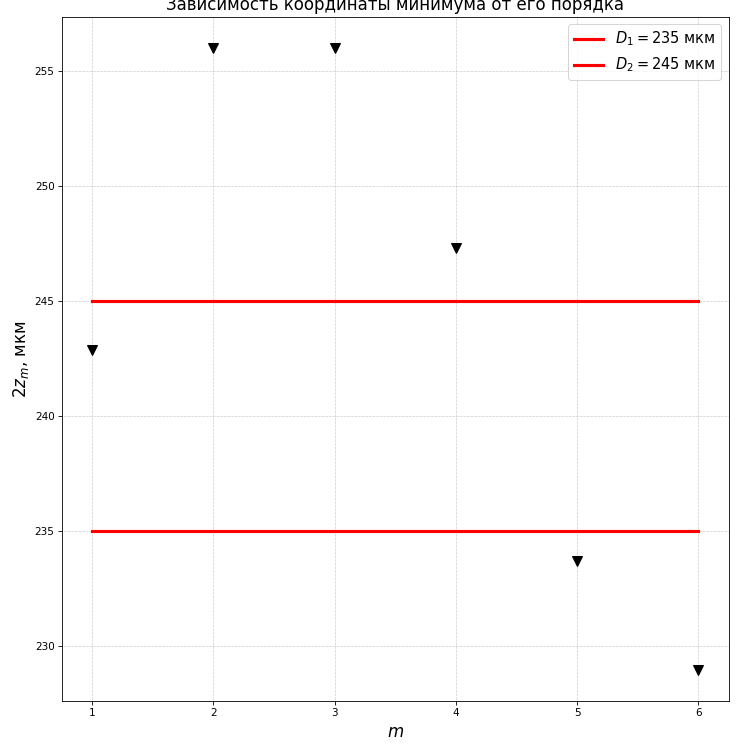
\includegraphics[width = \textwidth]{2z(m).png}
\end{figure}
\[D_{aver} = (244,1 \pm 4,6)\text{ мкм}\]
Погрешность среднего можно рассчитать по формуле
\[\sigma_{D_{aver}}^2 = \frac{\sum (D_i - D_{aver})^2}{n(n-1)}\]

\newpage
\begin{figure}[H]\label{fig: Fraunhofer, X_m(m)}
    \centering
    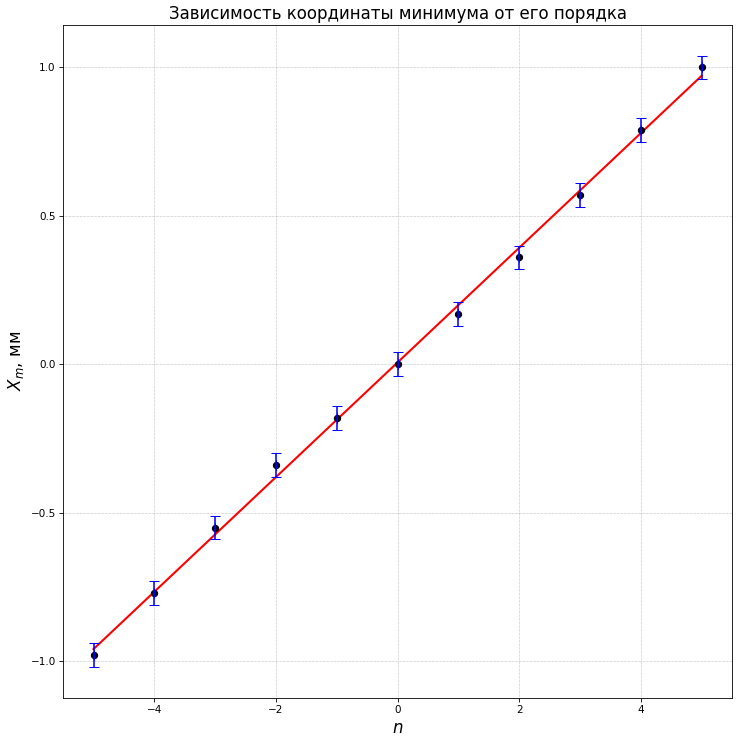
\includegraphics[width = \textwidth]{x_m(m).png}
\end{figure}
\[k = (19,3 \pm 0,2)\cdot 10^{-2} \text{ мм}, \quad \varepsilon_k = 1,17\%\]

\newpage

%%%%%%%%%%%%%%%%%%%%%%%%%
\end{document}
